% Template for PLoS
% Version 3.4 January 2017
\documentclass[10pt,letterpaper]{article}
\usepackage[top=0.85in,left=2.75in,footskip=0.75in]{geometry}

% amsmath and amssymb packages, useful for mathematical formulas and symbols
\usepackage{amsmath,amssymb}

% Use adjustwidth environment to exceed column width (see example table in text)
\usepackage{changepage}

% Use Unicode characters when possible
\usepackage[utf8x]{inputenc}

% textcomp package and marvosym package for additional characters
\usepackage{textcomp,marvosym}

% cite package, to clean up citations in the main text. Do not remove.
% \usepackage{cite}

% Use nameref to cite supporting information files (see Supporting Information section for more info)
\usepackage{nameref,hyperref}

% line numbers
\usepackage[right]{lineno}

% ligatures disabled
\usepackage{microtype}
\DisableLigatures[f]{encoding = *, family = * }

% color can be used to apply background shading to table cells only
\usepackage[table]{xcolor}

% array package and thick rules for tables
\usepackage{array}

% create "+" rule type for thick vertical lines
\newcolumntype{+}{!{\vrule width 2pt}}

% create \thickcline for thick horizontal lines of variable length
\newlength\savedwidth
\newcommand\thickcline[1]{%
  \noalign{\global\savedwidth\arrayrulewidth\global\arrayrulewidth 2pt}%
  \cline{#1}%
  \noalign{\vskip\arrayrulewidth}%
  \noalign{\global\arrayrulewidth\savedwidth}%
}

% \thickhline command for thick horizontal lines that span the table
\newcommand\thickhline{\noalign{\global\savedwidth\arrayrulewidth\global\arrayrulewidth 2pt}%
\hline
\noalign{\global\arrayrulewidth\savedwidth}}


% Remove comment for double spacing
%\usepackage{setspace}
%\doublespacing

% Text layout
\raggedright
\setlength{\parindent}{0.5cm}
\textwidth 5.25in
\textheight 8.75in

% Bold the 'Figure #' in the caption and separate it from the title/caption with a period
% Captions will be left justified
\usepackage[aboveskip=1pt,labelfont=bf,labelsep=period,justification=raggedright,singlelinecheck=off]{caption}
\renewcommand{\figurename}{Fig}

% Use the PLoS provided BiBTeX style
% \bibliographystyle{plos2015}

% Remove brackets from numbering in List of References
\makeatletter
\renewcommand{\@biblabel}[1]{\quad#1.}
\makeatother

% Leave date blank
\date{}

% Header and Footer with logo
\usepackage{lastpage,fancyhdr,graphicx}
\usepackage{epstopdf}
\pagestyle{myheadings}
\pagestyle{fancy}
\fancyhf{}
\setlength{\headheight}{27.023pt}
\lhead{
\includegraphics[width=2.0in]{PLOS-submission.eps}}
\rfoot{\thepage/\pageref{LastPage}}
\renewcommand{\footrule}{\hrule height 2pt \vspace{2mm}}
\fancyheadoffset[L]{2.25in}
\fancyfootoffset[L]{2.25in}
\lfoot{\sf PLOS}

%% Include all macros below
\newcommand{\lorem}{{\bf LOREM}}
\newcommand{\ipsum}{{\bf IPSUM}}


\usepackage{threeparttable}
\usepackage[table]{xcolor}
\usepackage{graphicx}
\usepackage{tabularx}
\usepackage{longtable}
\usepackage{siunitx}



\usepackage{forarray}
\usepackage{xstring}
\newcommand{\getIndex}[2]{
  \ForEach{,}{\IfEq{#1}{\thislevelitem}{\number\thislevelcount\ExitForEach}{}}{#2}
}

\setcounter{secnumdepth}{0}

\newcommand{\getAff}[1]{
  \getIndex{#1}{YORK,MANSOURA}
}

\providecommand{\tightlist}{%
  \setlength{\itemsep}{0pt}\setlength{\parskip}{0pt}}

\begin{document}
\vspace*{0.2in}

% Title must be 250 characters or less.
\begin{flushleft}
{\Large
\textbf\newline{Motor Learning Without Moving: Proprioceptive and Predictive Hand
Localization After Passive Visuoproprioceptive Discrepancy Training} % Please use "sentence case" for title and headings (capitalize only the first word in a title (or heading), the first word in a subtitle (or subheading), and any proper nouns).
}
\newline
\\
Ahmed A. Mostafa\textsuperscript{\getAff{YORK}, \getAff{MANSOURA}},
Bernard Marius 't Hart\textsuperscript{\getAff{YORK}}\textsuperscript{*},
Denise Y.P. Henriques\textsuperscript{\getAff{YORK}}\\
\bigskip
\textbf{\getAff{YORK}}CVR / Kinesiology and Health Science, York University, Toronto, Ontario,
Canada\\
\textbf{\getAff{MANSOURA}}Faculty of Physical Education, Mansoura University, Mansoura, Egypt\\
\bigskip
* Corresponding author: thartbm@gmail.com\\
\end{flushleft}
% Please keep the abstract below 300 words
\section*{Abstract}
An accurate estimate of limb position is necessary for movement
planning. Where we localize our unseen hand after a reach depends on
felt hand position, or proprioception, but this is usually neglected in
favour of predicted sensory consequences based on efference copies of
motor commands. Both sources of information should contribute, so here
we set out to further investigate how much of hand localization depends
on proprioception and how much on predicted sensory consequences. We use
a passive training paradigm with rotated visual feedback that eliminates
the possibility to update predicted sensory consequences, but still
recalibrates proprioception. After this training we measure
participants' hand location estimates based on both efference-based
predictions and afferent proprioceptive signals with self-generated hand
movements as well as based on proprioception only with robot-generated
movements. We find indistinguishable shifts in hand localization after
robot- and self-generated hand movements, and changes in open-loop
reaches. Both motor and proprioceptive changes are only slightly smaller
as those after training with self-generated movements, confirming that
proprioception plays a large role in estimating limb position and in
planning movements. (data: https://doi.org/10.17605/osf.io/zfdth,
preprint: https://doi.org/10.1101/384941)

% Please keep the Author Summary between 150 and 200 words
% Use first person. PLOS ONE authors please skip this step.
% Author Summary not valid for PLOS ONE submissions.

\linenumbers

% Use "Eq" instead of "Equation" for equation citations.
\section{Introduction}\label{introduction}

Sensory information is central to how we control all our movements. Our
brain is even thought to use predicted sensory consequences derived from
efferent copies of motor commands for motor control {[}1{]}. When
training with rotated visual feedback of the hand, we update these
predictions {[}2{]}. Additionally, such training leads to a
recalibration of our sense of felt hand position - ``proprioception'' -
to be more aligned with the distorted visual feedback {[}3{]}. Both of
these changes have been measured by asking people to localize where
their unseen hand is -- before and after training {[}4--8{]}. While our
lab has previously found that proprioception accounts for a large
portion of the change in hand localization {[}9{]}, it is far from clear
how much each process contributes or how to tease them apart. Here we
use passive training, that removes the need to update predicted sensory
consequences, in an attempt to isolate the contribution of
proprioception to hand localization.

The predicted sensory consequences of movements may play several
important roles in motor learning and control. Predicted sensory
consequences allow us to correct our movements before sensory error
signals are available, they can be used to select movements that best
achieve our goals and they may inform us on the location of our limbs.
Hence measuring predicted sensory consequences is valuable in movement
research. In visuomotor rotation adaptation tasks, the actual sensory
outcome is systematically different from the expected outcome, so that
participants update their predictions on the outcome of the trained
movements. In previous experiments, people were asked to make a movement
and then indicate the location of, or ``localize,'' their unseen, right
hand, before and after training with rotated visual feedback {[}5,7{]}.
Since there was no visual information available to the participants, the
predicted sensory consequences of the movement should be used in
localizing the unseen hand. Both studies found a significant shift in
hand localization, providing evidence that predicted sensory
consequences are indeed updated as a result of visuomotor rotation
adaptation.

However, our lab has shown that our sense of where we feel our hand to
be, proprioception, is also reliably recalibrated after visuomotor
rotation adaptation {[}3,9--18{]}. This has also been shown by other
labs {[}19{]} and a comparable proprioceptive change is induced with
force-field adaptation {[}20{]}. As proprioception also informs us on
the location of our limbs, we have on occasion used a task that is very
similar to hand localization to investigate this {[}3,6,21,22{]}.
Although proprioceptive recalibration has been largely ignored as an
explanation for changes in hand localization, we and others have shown
that it accounts for a substantial part of the changes in localization,
along with updates in predicted sensory consequences {[}9,19{]}.
Nevertheless, it is far from clear how much proprioception and
prediction each contribute to hand localization.

Here we intend to further examine the contribution of proprioception to
hand localization. To do this, we use passive training, where a robot
arm moves the participant's arm out, so that the cursor always directly
goes to the target {[}19,23,24{]}. This means there is no efference copy
available and no visuomotor error-signal, both of which are required to
update predicted sensory consequences. However, we impose a discrepancy
between vision and proprioception that drives proprioceptive
recalibration. Thus, changes in hand localization after this type of
training should be due to proprioceptive recalibration only. We use the
same experimental protocol as before {[}9{]}, so that we can compare
localization shifts between the two different types of training, and can
better assess the contributions of predicted sensory consequences and
proprioception to hand localization.

\section{Methods}\label{methods}

We set out to test the relative contributions of proprioception and
efference-based prediction to hand localization. We use visual training
with robot-generated hand movements to prevent updates of predicted
sensory consequences, but still elicit proprioceptive recalibration.

\subsection{Participants}\label{participants}

Twenty-five right-handed participants were recruited for this study. One
participant was excluded for not following task instructions, and three
were excluded for low performance on a task that ensures attention
during the passive training. All analyses presented here pertain to the
remaining twenty-one participants (13 females and 8 males, mean age:
20.1 +/- 2.3 years), but the data of the three low-performing
participants is included in the online
\href{https://osf.io/zfdth}{dataset} {[}25{]}. All had normal or
corrected-to-normal vision, and provided prior, written informed consent
in accordance with the ethical guidelines set by the York Human subjects
Review Subcommittee and received credit toward an undergraduate
psychology course. Participants were screened verbally, and all reported
being right handed and not having any history of visual, neurological,
and/or motor dysfunction.

\begin{figure}
\centering
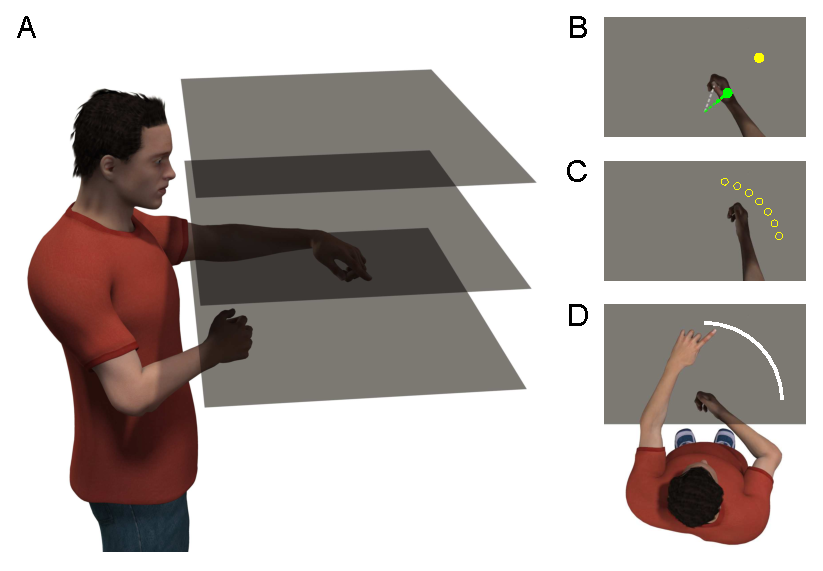
\includegraphics{Fig1_setup.eps}
\caption{\textbf{Setup and tasks:} \textbf{a)} Participants moved their
unseen right hand with visual feedback on hand position provided through
a mirror (middle surface) half-way between their hand and the monitor
(top surface). A touchscreen located just above the hand was used to
collect responses for the localization tasks (bottom surface).
\textbf{b)} Training task. The target, shown as a yellow disc, is
located 10 cm away from the home position at 45°. In the rotated
training tasks, the cursor (shown here as a green circle) represents the
hand position rotated 30° relative to the home position. \textbf{c)}
No-cursor reach task. Targets are located 10 cm away from the home
position at 15°, 25°, 35°, 45°, 55°, 65°, and 75°, shown by the yellow
circles here (only one was shown on each trial). While reaching to one
of these targets, no visual feedback on hand position is provided. d)
Localization task. The participants' unseen, right hands moved out, and
subsequently participants indicated the direction of the hand movement
by indicating a location on an arc using a touch screen with their
visible left index finger}
\end{figure}

\subsection{Setup}\label{setup}

Participants sat in a height-adjustable chair to ensure that they could
easily see and reach all targets presented on a reflective screen (see
Fig 1). During all tasks, they held the vertical handle on a two-joint
robot manipulandum (Interactive Motion Technologies Inc., Cambridge, MA)
with their right hand so that their thumb rested on top of the handle. A
monitor (Samsung 510 N, refresh rate 60 Hz) was mounted 11 cm above the
reflective screen, such that images displayed on the monitor appeared to
lie in the horizontal plane where the right hand was moving. The
reflective screen was mounted horizontally 18 cm above the robot
manipulandum. A touch screen was mounted 13 cm underneath the reflective
surface, so that subjects could indicate the location of the unseen
right-hand locations (specifically the unseen thumb) with their visible
left hand, which was lit up with a small spot light (only in
localization tasks). The room lights were dimmed and the participants'
view of their right hand was blocked by the reflective screen, as well
as a dark cloth draped between the touch screen and participants' right
shoulders.

\subsection{Procedure}\label{procedure}

The first part of the experiment used training with a cursor aligned
with the hand and the second part had training with a cursor rotated
around the start position (Fig 1b; white rows in Table 1). During the
training with rotated feedback, the cursor was gradually rotated 30°
clockwise. This introduced a discrepancy between the actual, or felt,
hand position and the visual feedback, that should evoke proprioceptive
recalibration. However, the movements were robot generated, so that
there were no predicted sensory consequences based on the outgoing motor
command. Hence the prediction errors that are thought to lead to motor
learning were absent as well. After both types of training, participants
did open-loop reaches as well as two kinds of hand localization tasks,
to test the effect of training on proprioceptive and predictive hand
estimates.

\newcommand{\headrow}{\rowcolor{black!20}}
\newcommand{\thead}[1]{\multicolumn{1}{l}{\bfseries #1\rule[-1.2ex]{0pt}{2em}}}

\definecolor{LGray}{gray}{0.9} \definecolor{DGray}{gray}{0.8}

\begin{table}[bt]
\caption{Task order}
\begin{threeparttable}
\begin{tabular}{cccc}
\headrow
\multicolumn{2}{c}{\# trials} & \multicolumn{2}{c}{training type} \\
\headrow
%\multicolumn{2}{|c|}{\# trials} & \thead{Exposure training} & \thead{Classic training} \\
\thead{aligned} & \thead{rotated} & \multicolumn{1}{c}{\textbf{Exposure training}} & \multicolumn{1}{c}{\textbf{Classic training}} \\
\rowcolor{white}
50 & 90 & training & training \\
\rowcolor{LGray}
- & 21 & no-cursor & no-cursor \\
\rowcolor{white}
- & 60 & training & training \\
\rowcolor{DGray}
25 & 25 & active delayed localization & active delayed localization \\
\rowcolor{LGray}
21 & 21 & no-cursor & no-cursor \\
\rowcolor{white}
10 & 60 & training & training \\
\rowcolor{DGray}
25 & 25 & passive delayed localization & passive delayed localization \\
\rowcolor{LGray}
21 & 21 & no-cursor & no-cursor \\
\rowcolor{white}
10 & 60 & training & training \\
\rowcolor{DGray}
25 & 25 & active delayed localization & \textit{(active online localization)} \\
\rowcolor{LGray}
21 & 21 & no-cursor & no-cursor \\
\rowcolor{white}
10 & 60 & training & training \\
\rowcolor{DGray}
25 & 25 & passive delayed localization & \textit{(passive online localization)} \\
\rowcolor{LGray}
21 & 21 & no-cursor & no-cursor \\
\hiderowcolors
\hline  % Please only put a hline at the end of the table
\end{tabular}

\begin{tablenotes}
\item 
\end{tablenotes}
\end{threeparttable}
\end{table}

\subsection{Exposure training}\label{exposure-training}

In what we call `exposure training' the participants did not move their
hand toward the target, but the robot did. In this task (Table 1), the
right hand was represented by a cursor (green disk, 1 cm in diameter,
Fig 1b) located directly above participant's thumb. The robot moved the
participant's unseen right hand (and the cursor) along a direct path
toward a visual yellow target disk and back to the starting position (1
cm in diameter, Fig 1b). The home position was located approximately 20
cm in front of participants and the visual target located 10 cm from the
home position at 45° (Fig 1b). In order to make sure participants were
paying attention to the cursor, the cursor was switched off for 2 screen
refreshes (\textasciitilde{}33.3ms) on 50\% of the trials at a random
distance between 4 and 9 cm from the home position and participants were
asked to report this using a button press with the left hand.
Performance on this task was used to screen participants.

During the first half of the experiment, the cursor and hand path were
aligned during exposure training. In the second part of the experiment,
the ``rotated'' session, the same visual training target at 45° was
used, and the cursor kept moving straight to this target. However, the
robot-generated hand path gradually rotated 30° CCW (Fig 1b) with
respect to the visible target and the cursor in increments of
0.75°/trial, so that the full rotation was reached after 45 trials. This
mimicked error-free responses to a gradual visuomotor rotation of 30°
CW. The initial training consisted of 50 trials in the aligned part and
90 in the rotated part. In between open-loop reach tasks and
localization tasks (Table 1) extra training tasks were done, each of
which consisted of 10 trials in the aligned part of the experiment and
60 trials in the rotated part (Table 1).

\subsection{No-cursor reaching}\label{no-cursor-reaching}

The trials in no-cursor reaching (Table 1, light gray rows) serve as a
classical measure of motor adaptation. On each of these trials
participants were asked to reach with their unseen right hand to one of
7 visual targets, without any visual feedback of hand position. The
targets were 10 cm from the home position, located radially at: 15°,
25°, 35°, 45°, 55°, 65°, and 75° (Fig 1c). A trial started with the
robot handle at the home position and, after 500 ms, the home position
disappeared and the target appeared, cuing the participants to reach for
the target. Once the participants thought they had reached the target
they held their position for 250 ms, and the target and the home
position disappeared, cuing participants to move back to the home
position along a straight, constrained path, to begin the next trial. If
participants tried to move outside of the path, a resistance force, with
a stiffness of 2 N/(mm/s) and a viscous damping of 5 N/(mm/s), was
generated perpendicular to the path. In every iteration of the no-cursor
reach task, each target was reached three times, for a total of 21
reaches in pseudo-random order. The no-cursor reaching task was
performed four times in the aligned part of the experiment and five
times in the rotated part of the experiment.

\subsection{Localization}\label{localization}

In this task (Fig 1d; Table 1, dark gray rows) participants indicated
where they thought their unseen right hand was after a movement. First,
an arc appeared, spanning from 0° to 90° and located 10 cm away from the
home position and the participants' unseen, right hand moved out from
the home position in a direction towards towards a point on the arc. The
hand was stopped by the robot at 10 cm from the home position and then,
to prevent the online proprioceptive signals from overriding the
predictive signals {[}5,9{]}, the hand was moved back to the home
position using the same kind of constrained path as used for the return
movements in the no-cursor task. Participants indicated with the index
finger of their visible, left hand on the touch screen mounted directly
above the robot handle where they thought their trained hand had crossed
the arc.

Crucially, there were two variations of this task. First, in the
`active' localization task participants generated the movement
themselves, as they could freely move their unseen right hand from the
home position to any point on the arc. Second, there was a `passive'
localization task where the robot moved the participants' hand out and
back, to the same locations the participants moved to in the preceding
`active' localization task in a shuffled order (hence, active
localization is done first). In active localization, participants have
access to both proprioceptive information as well as an efference-based
prediction of sensory consequences, but in passive localization, only
proprioception should be available. The active and passive localization
task each consisted of 25 trials, and each of the tasks was done a total
of four times; twice after aligned and twice after rotated training.

\subsection{Classic training}\label{classic-training}

The paradigm described above is an exact replica of a paradigm we used
earlier {[}9{]} with two exceptions. First, we used exposure training
here, instead of the standard reach training with volitional movements,
which we will call `classic' training. Second, all localization is
delayed until the right hand has returned to the home position in this
study (see Table 1), so that instead of both delayed and online
localization we have two repetitions of each delayed localization task.
With this paradigm we can compare changes in localization and no-cursor
reaches change after exposure training with changes in the same measures
after classic visuomotor adaptation training.

\subsection{Analyses}\label{analyses}

Prior to any analyses, both the localization responses and the no-cursor
reach data were visually inspected and trials where the participants did
not follow task instruction were removed (e.g.~several movements back
and forth, or a touch-screen response on the home position, instead of
on the white arc).

\subsection{Localization}\label{localization-1}

Localization responses were taken as the (signed) angular difference
between vectors through the home position and the actual hand position
as well as the location indicated on the touch screen. Prior to
analyses, idiosyncratic differences in performing this task were
countered. Before conversion to degrees angle, a circle with a 10 cm
radius was fit to the touch screen responses of each participant and the
offset of this circle's centre was subtracted from all response
coordinates, so that all responses fell close to the arc. Then, a
smoothed spline was fit to every participant's response errors in each
of the four localization tasks (aligned vs.~rotated and active
vs.~passive) and these were used to obtain localization errors at the
same locations used for the no-cursor reaches (15°, 25°, 35°, 45°, 55°,
65° and 75°), but only if that location fell within the range of the
data (i.e.~we only interpolate). This way localization responses could
be compared across participants despite the freely chosen reach
directions. At the 15° location 7/21 participants didn't have an
estimate in one or more of the four localization tasks (in the
``classic'' data it was also 7/21). While that data is shown in the
figures, we did not use it for analysis.

First we test if localization responses shifted following rotated
exposure training compared to aligned. We then test if the shift in
localization responses is different for active and passive localization,
and we run analyses comparing localization after exposure training with
localization after ``classic'' training. Finally, we explore the
generalization of localization responses and if they are different
between the groups doing classic and exposure training.

\subsection{Reach aftereffects}\label{reach-aftereffects}

To assess any reach adaptation that may have occurred after exposure
training we analyzed reach endpoint errors in no-cursor trials. Reach
endpoint errors were the (signed) angular difference between a vector
from the home position to reach endpoint and a vector from the home
position to the target. We obtained reach aftereffects by subtracting
reach endpoint errors after aligned training from those after rotated
training. No-cursor endpoint errors were analyzed to see if participants
adapted the direction of their reaching movements after rotated exposure
training. We also tested if any such change decayed, i.e.~if it was the
same immediately after exposure training, or when a localization task
was done in between exposure training and no-cursor reaches.
Furthermore, we tested if the generalization of reach aftereffects is
different between exposure and classic training and if there is any
generalization of reach aftereffects.

Pre-processing and analyses were done in R 3.4.4 {[}26{]}, using lme4,
lmerTest and various other packages. Most analyses used linear mixed
effects models, since there is some missing localization data. These
were ``converted'' to more readable ANOVA-like output, using a
Satterthwaite approximation {[}27{]}. Highly similar results were
obtained with a Chi-square approximation. Data, scripts and a notebook
with analyses have been made available on the Open Science Framework
{[}25{]} (\href{https://osf.io/zfdth/}{https://osf.io/zfdth}).

In short, this experiment allowed us to test how mere exposure to a
visual-proprioceptive discrepancy changes both reach aftereffects and
hand localization responses, and compare them with those obtained after
more regular, ``classic'' training.

\section{Results}\label{results}

In this study we intend to further elucidate the relative contributions
of (updated) predicted sensory consequences and (recalibrated)
proprioception to hand localization. We can parcel out these
contributions by measuring hand localization after both robot-generated
and self-generated movements. Finally we compare the data from the
current experiment with those obtained in an earlier study that used an
identical paradigm, but trained with self-generated movements, or
``classic'' training.

\begin{figure}
\centering
\includegraphics{Fig2_plain.pdf}
\caption{\textbf{Hand localization:} The shifts of the angles of
touchscreen responses in all variations of the localization task, using
spline-interpolated estimates for hand angles matching the reach targets
in the no-cursor reach block. \textbf{a)} Localization shifts after
exposure training. Dark blue: active localization shifts, Light blue:
passive localization shifts. \textbf{b)} Localization shifts after
classic training. Dark red: active localization shifts, Orange: passive
localization shifts. The dashed line segments illustrate that the 15°
data is not used for statistical analyses (see Methods). \textbf{c)}
Generalization curves of active localization shifts after exposure
training (blue) and classic training (red). Shaded areas: 95\%
confidence intervals for the peak of the generalization curve (red and
blue lines through shaded area indicate 50\% points). Downward black
arrow: visual trained target. Upward black arrow: hand location during
training.}
\end{figure}

\subsection{Localization}\label{localization-2}

Here we test our hypothesis that exposure training does not lead to
changes in predicted sensory consequences. Since the difference between
active and passive localization stems only from the presence or absence
of predicted sensory consequences, there should be no difference between
the two if predicted sensory consequences are not changed by exposure
training. At first glance, it seems there might be a difference between
active and passive localization shifts in exposure training (see Fig
2a), although it is smaller than in classic training (Fig 2b).

To test if rotated exposure training induces changes in hand
localization, we fit an LME to the localization errors throughout the
workspace using session (aligned or rotated), movement type (active and
passive) and hand angle (25°, 35°, 45°, 55°, 65° and 75°), and all
interactions as fixed effects and participant as random effect. There
was an effect of session (F(1,450.5)=155.8; p\textless{}0.001), showing
that exposure training leads to changes in hand localization. There was
also an effect of hand angle (F(5,450.6)=6.54; p\textless{}.001) and an
interaction between hand angle and session (F(5,450.3)=8.25;
p\textless{}.001), which we'll explore below, but no other effects (all
p\textgreater{}.60). Since localization responses did shift, we use the
difference between hand localization after rotated training and after
aligned training (as plotted in Fig 2) for further tests.

If this shift in localization after exposure training partly reflects
predicted sensory consequences, then shifts in active localization, that
rely on both (recalibrated) proprioception and (updated) predictions
should be different from shifts in passive localization that only rely
on (recalibrated) proprioception. We fit an LME to the change in
localization using movement type (active or passive localization) and
hand angle, as well as their interaction as fixed effects and
participant as random effect. There was no effect of movement type
(F(1,211.8)=0.07; p=0.79). There was an effect of hand angle
(F(5,212.2)=10.8; p\textless{}0.001), but no interaction between hand
angle and movement type (F(5,211.8)=1.23, p=.29). The lack of an effect
of movement type suggests that predicted sensory consequences did not
contribute to localization in this paradigm.

In order to compare hand localization shifts after exposure training
with those after classic training {[}9{]}, we fit an LME to localization
shift using training type (exposure vs.~classic), movement type (active
vs.~passive) and hand angle and all interactions as fixed effects and
participant as random effect. There was a main effect of movement type
(F(1,422.0)=6.22; p=.013) and of hand angle (F(5,422.7)=8.19;
p\textless{}.001), as well as an interaction between training type and
hand angle (F(5,422.7)=4.54; p\textless{}.001) and between training type
and movement type (F(1,422.0)=4.48, p=.035), but there was no main
effect of training type (F(1,39.1)=0.92, p=.34) and no other effects
(all p\textgreater{}.14). These results also suggest that the magnitude
of the shifts in localization are comparable between classic and
exposure training, but that the pattern of generalization is different.

To address our main question, we will look at the interaction between
training type (exposure vs.~classic) and movement type (active
vs.~passive) we found above. Since there is no difference between active
and passive localization shifts after exposure training alone, the
interaction between training type and movement type should be caused by
an effect of movement type on the localization shifts after classic
training, as we found previously {[}9{]}. This means that shifts in hand
localization after exposure training indeed rely on recalibrated
proprioception alone, while after classic training, there also is a
contribution of predicted sensory consequences to active localization.

For completeness, we explore the potentially different generalization
patterns of localization shifts after classic and exposure training (Fig
2c). The LME indicates no difference in overall amplitude of
localization shifts between the groups, so the interaction between
training type and hand angle might stem from a generalization that does
not peak at the trained location after exposure training. Using the
active localization shifts only (which are larger, and arguably more
similar to reach aftereffects), we bootstrap a 95\% confidence interval
for the peak localization shift across participants in each group. Here
we include the data at 15° where it is available. After classic
training, the peak localization shift was at 48.8° (95\% confidence:
31.6° - 62.8°; red area in Fig 2c), and after exposure training the peak
localization shift was at 62.1° (95\% confidence: 50.0° - 75.6°; blue
are in Fig 2c). This means that peak localization after classic training
is lower than after exposure training, but not vice versa. Also note
that the confidence interval for the peak localization shift after
classic training includes the trained target (45°), but not after
exposure training {[}5{]}. In short, the LME for localization shifts
indicates a different generalization curve after exposure and classic
training, which might be partially explained by a different position of
the peak localization shift after exposure or classic training.

\subsection{Reach aftereffects}\label{reach-aftereffects-1}

Apart from proprioception and prediction, we want to see if rotated
exposure training has any effect on open-loop reaches and if these are
robust. We measure whether participants adapted their reach directions
by assessing their reach errors in no-cursor reach trials after aligned
and rotated exposure training. In Fig 3, the changes in no-cursor
endpoint errors, or reach aftereffects, appear to be well over 5°.
First, to test if exposure training affects open-loop reach direction,
we fit a linear mixed effects model (LME) to reach endpoint error using
session (aligned; all blocks, or rotated; only the first block
immediately after training) and target (15°, 25°, 35°, 45°, 55°, 65° and
75°), as well as their interactions as fixed effects and participant as
random effect. There is an effect of session (F(1,260)=93.81,
p\textless{}.001), that is: exposure training leads to substantial reach
aftereffects. There was no effect of target (F(6,260)=1.07, p=.37) and
no interaction (F(6,260)=1.00, p=.42). Since there is an effect of
session, we now take the differences in reach endpoint errors between
the rotated and aligned session for every participant and target as
reach aftereffects, and use those for all further analyses.

\begin{figure}
\centering
\includegraphics{Fig3_plain.pdf}
\caption{\textbf{Reach aftereffects:} Changes of the angle of reach
endpoints in the no-cursor tasks. \textbf{a)} Reach aftereffects across
the experiment. Light blue: first no-cursor task in the rotated session
(immediately following training), Dark blue, dashed line: the other four
repetitions of the task (with localization in between training and
no-cursor tasks). \textbf{b)} Reach aftereffects after classic and
exposure training. Blue: exposure training, Red: classic training.
\textbf{c)} Generalization curves of reach aftereffects after exposure
training (blue) and classic training (red). Shaded areas: 95\%
confidence intervals for the peak of the generalization curve (red and
blue lines through shaded area indicate 50\% points). Downward black
arrow: visual trained target. Upward black arrow: hand location during
training.}
\end{figure}

To see if reach aftereffects decayed during the localization tasks, we
compared reach aftereffects in the initial no-cursor block, that
immediately followed training, with those in the later blocks that
followed a localization task. We fit an LME to the reach aftereffects
with iteration (initial vs.~later no-cursor blocks) and target (as
above) as well as their interaction as fixed effects and participant as
random effect. There is no effect of iteration (F(1,260)=2.72, p=0.10).
There was an effect of target (F(6,260)=6.29, p\textless{}.001) but no
interaction (F(6,260)=0.58, p=0.74). Hence, reach aftereffects were not
appreciably different right after training and after the localization
tasks. In other words, there was likely no noticeable decay of reach
aftereffects during the localization tasks, so that we can collapse the
data across iterations.

Next we compare the reach aftereffects after classic training with those
after exposure training (Fig 3b). It appears as if there is little
overall difference in magnitude, but there might be a shift of the
generalization curve. We fit an LME to reach aftereffects with training
type (classic vs.~exposure), target (as above) as well as their
interaction as fixed effects and participant as random effect. There is
no main effect of training (F(1,40)=0.11, p=.74), indicating
approximately equal magnitude of reach aftereffects after the two
training types. There is an effect of target (F(6,240)=8.36,
p\textless{}.001), indicating that reach aftereffects exhibit some form
of a generalization curve. There is also an interaction between training
type and target (F(6,240)=2.27, p=.038), indicating these generalization
curves are different after the two training types.

We will explore these potentially different generalization curves here.
In Fig 3c we can observe that reach aftereffects after exposure training
seem not to peak at the trained target direction of 45° but a more
forward direction. We test this by taking the 95\% confidence interval
of the centre of a normal curve fit to this data, bootstrapped across
participants, and find that the median peak of the generalization curve
of reach aftereffects after exposure training is at 66.3°, with a 95\%
confidence interval ranging from 49.3° to 78.9°. This would indeed
suggest that the reach aftereffects after exposure training do not
generalize around the trained direction of 45°, but at a more counter
clockwise location. For classic training, generalization of reach
aftereffects peaks at 53.2°, with a 95\% confidence interval spanning
42.1° to 66.5°. So for classic training the 95\% confidence interval for
peak reach aftereffects does include the trained target. These
confidence intervals also indicate that generalization of reach
aftereffects does not peak at different target position after exposure
and classic training. However, we can also observe that the full curve
was not sampled after exposure training, so that curve fitting is not
optimal. This means that -- given our data -- the interaction between
target and training type found in the LME above can't be explained by a
shifted generalization curve. This may be because our experiment was not
set up to test this, and the similar angles where generalization peaks
in both localization and reach aftereffects, suggests there may be a
difference in where proprioception and prediction generalize strongest.

In summary, our main hypotheses are confirmed; exposure training leads
to shifts in hand localization that are not different for active or
passive localization, while movement type does have an effect on
localization shift after classic training. Exposure training also causes
robust reach aftereffects that are of comparable size to those found
with classic training. There is some evidence that the generalization of
both localization shifts and reach aftereffects are different after the
two training types, and it appears this can partially be explained by a
different peak of the generalization curves, but our data and analyses
are not definitive.

\section{Discussion}\label{discussion}

The position of limbs is important for planning and evaluating
movements, and can be estimated through predicted sensory consequences,
as well as visual and proprioceptive feedback. As in a previous study
{[}9{]} here we quantify the contributions of predicted sensory
consequences and proprioceptive recalibration to where we localize our
hand after training with altered visual feedback of the hand. In
classical adaptation paradigms, both predictions are updated and
proprioception is recalibrated. Predictions are updated when they don't
match actual sensory consequences, and proprioception is recalibrated
when it doesn't match visual feedback. In this study we use ``exposure''
training, where the participants do not have volitional control of their
movements. By design, this should eliminate efference copies and prevent
updating predicted consequences of movements, but since the
proprioceptive and visual feedback is the same, exposure training still
allows proprioceptive recalibration. Before and after training,
participants localize their hand, both after ``active,'' self-generated
movements that allow using predicted sensory consequences, and after
``passive,'' robot-generated movements that only allow using
proprioception. We calculate the training-induced shift in both types of
localization given the same actual hand position. After classical
training we previously reported larger shifts in active localization as
compared to passive {[}9{]}. As we expected, after exposure training
there are substantial shifts in localization, but no difference between
active and passive localization, indicating that predictions are not
updated after exposure training. Furthermore, we find that exposure
training evokes substantial and robust reach aftereffects, indicating
that recalibrated proprioception is used to plan movements.

Our lab previously investigated proprioceptive recalibration and reach
aftereffects following visuomotor adaptation with classic training and
matched exposure training. There we also found that proprioceptive
recalibration is of similar magnitude in both training paradigms, but
unlike here, reach aftereffects are usually much larger with classic
training {[}13,18,22--24{]}. And while proprioceptive recalibration and
reach aftereffects do proportionally increase with gradual increases in
rotation size for classical training, they do not for exposure training
{[}24{]}. The similar magnitude of proprioceptive recalibration and
reach aftereffects following exposure training, but not classical
training, suggest that this sensory recalibration is partly driving this
modest change in movements. The effect of exposure training on movements
is also demonstrated by facilitation by exposure training of subsequent
classic training {[}28{]} (but no interference) and transfer of exposure
training effects from one hand to the other {[}29{]}. In the current
study, we further demonstrate that exposure training affects movements
and proprioception, but also measure its potential effect on predictive
estimates.

Results similar to what we find here were reported in a study by Cameron
and colleagues {[}19{]}, using gain modulation of visual feedback of
single-joint hand movements around the elbow. Their within-subjects
experiment included both training with volitional movements as well as
with passive movements and also tested perception of movements that were
either passive or active. They too found a robust change in passive
perception of hand movement (using a different measure), and these
changes did not differ between the two types of training. Similarly,
they found shifts in what we might call ``active localization,''
although the task is different, after both training types. Like here,
these shifts are larger after classic training as compared to exposure
training. They also found that passive exposure leads to reach
aftereffects, although these were smaller than those produced following
``classical'' training with altered visual gain. Both our findings, and
those of Cameron et al. {[}19{]} indicate that updating predicted
sensory consequences requires volitionally controlled movements that
lead to prediction errors, while proprioception recalibrates equally in
both types of training, and that recalibrated proprioception affects
open-loop reaches. Our combined results suggest that updates in
predicted sensory consequences only provide a partial explanation for
motor learning.

Two related concerns about exposure training and passive localization
are that the movements are not fully passive, so that efference-based
predictions are still generated or that predicted sensory consequences
are generated through another route. Cameron et al. {[}19{]} measured
muscle activity (EMG) during passive movements and found no difference
with stationary baseline muscle activity. This suggests that any
movements generated in a passive condition are subthreshold, minimizing
efference-based predictions. The brain areas generating predicted
sensory consequences could also rely on afferent signals. However, such
afferent signals are present in both active and passive movements, and
if they would result in the same predictions, there would be no
difference between active and passive localization after classic
training, and no difference between the effects of exposure and classic
training, and we find both are different. Hence, while we can not fully
exclude any predictive signals in passive localization or exposure
training, our data shows that any residual predictive signals in the
passive movements we used are qualitatively very different from normal
efference-based predicted sensory consequences.

In our classical training group, we not only see shifts for passive
localization but even larger shifts for active localization which is
consistent with a change in both proprioception and an update in
predictions. In our exposure training, we did not find a consistent
difference between active and passive localization, and none at the
trained direction. Assuming that predictions were not updated in
exposure training, a maximum likelihood estimate (MLE) or ``optimal
integration'' {[}30{]} would predict that active localization should
shift less than passive localization after exposure training. But of
course this is not the case in our findings (although it is the case for
Cameron et al.). This suggests that perhaps these two signals are not
optimally integrated which is consistent with our comparisons of the
variance between passive and active localization. In 't Hart and
Henriques {[}9{]}, we tested the prediction derived from MLE that hand
localization with two signals -- proprioception and prediction in active
localization -- should be more reliable, i.e.~have lower variance, than
hand localization with only one signal -- proprioception only in passive
localization. However, we found no difference in variance between active
and passive localization, and recently replicated this in a much larger
dataset {[}31{]}. Taken together, this suggests these different sources
of information about unseen hand location are not optimally integrated.
While localizing the unseen hand is less precise than locating (pointing
to) a remembered visual target or a seen and felt hand location, we find
that these bimodal estimates are rarely integrated optimally
{[}32--34{]}, although others have {[}35{]}. A more recent study
{[}36{]} has also shed doubt on whether ``optimal'' or ``Bayesian''
integration is used for locating the hand with two afferent signals.
Analogously, here we again can't find evidence that afferent and
efferent information combine as a maximum likelihood estimate.

It seems clear that the cerebellum plays a role in motor learning as it
appears to compute predicted sensory consequences, i.e.~it implements a
forward model {[}37--39{]}. People with cerebellar damage do worse on
motor learning tasks {[}40--43{]}, and show decreased shifts in hand
localization tasks following motor learning {[}5,7{]}. This highlights
that the cerebellum, and likely predicted sensory consequences, are
important for motor learning, but does not explain the remaining shifts
in hand localization. We previously found that proprioceptive
recalibration is intact in people with mild cerebellar ataxia and that
it is similar following exposure and classical training with a gradually
introduced cursor rotation {[}18{]}. The remaining changes in hand
localization found in cerebellar patients can be attributed to
recalibrated proprioception which should be intact {[}18{]}.
Analogously, here we show that in a paradigm that stops updates of
predictions of sensory consequences, as supposedly in people with
cerebellar damage, we still see substantial shifts in localization.
Again, the remaining localization shifts can be explained if, along with
predictions, the human brain uses afferent signals: recalibrated
proprioceptive estimates, to localize the hand.

\subsection{Generalization}\label{generalization}

We do find some evidence that, after exposure training, the
generalization curves for localization shifts are not centred on the
visual location of the trained target; they don't peak at 45° but at
\textasciitilde{}62°. In contrast, after classic training the peak of
the generalization curve does peak close to the training target. It is
possible that proprioceptive recalibration is not anchored to the visual
goal of the training task as it is not a requirement to feel your hand
at any specific point; rather, in classic training the visual cursor has
to be brought to a visual target to end a trial. While in exposure
training the movements are executed for the participants without error,
their task is still to pay attention to the visual cursor while it moves
to the visual target; there are no task demands on proprioception.
Although we can't substantiate this here, the generalization curves of
the reach aftereffects seem to mimic the generalization curves of
localization shifts, suggesting a relationship between changes in state
estimates and changes in movements. This needs to be tested further, but
if these effects are true, they may provide insight into how state
estimates are used to produce movements, and also may lead to a new
method to disentangle the influence of recalibrated proprioception and
more traditional updated internal models on motor changes, such as reach
aftereffects. Either way, even though the experiment was not designed to
investigate this, the shifted generalization curves of changes in
localization after classic and exposure training suggest they are
generated by different mechanisms. This is in line with our earlier
findings that proprioception generalizes differently from reach
adaptation {[}11{]}.

\subsection{Conclusion}\label{conclusion}

To sum up, after a training paradigm designed to prevent updating of
predicted sensory consequences but allow recalibration of
proprioception, we find substantial changes in where people localize
their hand. This means that recalibrated proprioceptive estimates can
explain shifts in hand localization. The distinct change in the
direction of open-loop reaches we observe here, suggests recalibrated
proprioception can contribute to motor adaptation in other contexts as
well. Finally, we have some evidence that after exposure training, the
shift in hand localization does not generalize around the trained target
location. All of this confirms that different mechanisms underlie
proprioceptive recalibration and motor adaptation.

\subsection{Acknowledgements}\label{acknowledgements}

This work was supported by a Canadian Network for Research and
Innovation in Machining Technology NSERC Operating grant (DYPH) and the
German Research Foundation (DFG) under grant no. HA 6861/2-1 (BMtH). The
funders had no role in study design, data collection and analysis,
decision to publish, or preparation of the manuscript. We thank
Shanaathanan Modchalingam for assistance in collecting the data.

\section*{References}\label{references}
\addcontentsline{toc}{section}{References}

\hypertarget{refs}{}
\hypertarget{ref-Duhamel1992a}{}
1. Duhamel J-R, Colby CL, Goldberg ME. The updating of the
representation of visual space in parietal cortex by intended eye
movements. Science. 1992;255: 90--92.
doi:\href{https://doi.org/10.1126/science.1553535}{10.1126/science.1553535}

\hypertarget{ref-Wolpert1995}{}
2. Wolpert DM, Ghahramani Z, Jordan MI. An internal model for
sensorimotor integration. Science. 1995;269: 1880--2.
doi:\href{https://doi.org/10.1126/science.7569931}{10.1126/science.7569931}

\hypertarget{ref-Cressman2009}{}
3. Cressman EK, Henriques DYP. Sensory recalibration of hand position
following visuomotor adaptation. Journal of Neurophysiology. 2009;102:
3505--3518.
doi:\href{https://doi.org/10.1152/jn.00514.2009}{10.1152/jn.00514.2009}

\hypertarget{ref-Clayton2013}{}
4. Clayton HA, Cressman EK, Henriques DY. Proprioceptive sensitivity in
ehlers-danlos syndrome patients. Experimental Brain Research. 2013;230:
311--321.
doi:\href{https://doi.org/10.1007/s00221-013-3656-4}{10.1007/s00221-013-3656-4}

\hypertarget{ref-Izawa2012b}{}
5. Izawa J, Criscimagna-Hemminger SE, Shadmehr R. Cerebellar
contributions to reach adaptation and learning sensory consequences of
action. Journal of Neuroscience. 2012;32: 4230--4239.
doi:\href{https://doi.org/10.1523/JNEUROSCI.6353-11.2012}{10.1523/JNEUROSCI.6353-11.2012}

\hypertarget{ref-Jones2012a}{}
6. Jones SAH, Fiehler K, Henriques DYP. A task-dependent effect of
memory and hand-target on proprioceptive localization. Neuropsychologia.
2012;50: 1462--1470.
doi:\href{https://doi.org/10.1016/j.neuropsychologia.2012.02.031}{10.1016/j.neuropsychologia.2012.02.031}

\hypertarget{ref-Synofzik2008}{}
7. Synofzik M, Lindner A, Thier P. The cerebellum updates predictions
about the visual consequences of one's behavior. Current Biology.
2008;18: 814--818.
doi:\href{https://doi.org/10.1016/j.cub.2008.04.071}{10.1016/j.cub.2008.04.071}

\hypertarget{ref-Yavari2016}{}
8. Yavari F, Mahdavi S, Towhidkhah F, Ahmadi-Pajouh M-A, Ekhtiari H,
Darainy M. Cerebellum as a forward but not inverse model in visuomotor
adaptation task: A tDCS-based and modeling study. Experimental Brain
Research. 2016;234: 997--1012.
doi:\href{https://doi.org/10.1007/s00221-015-4523-2}{10.1007/s00221-015-4523-2}

\hypertarget{ref-Hart2016}{}
9. 't Hart BM, Henriques DY. Separating predicted and perceived sensory
consequences of motor learning. PLoS ONE. 2016;11.
doi:\href{https://doi.org/10.1371/journal.pone.0163556}{10.1371/journal.pone.0163556}

\hypertarget{ref-Mostafa2014}{}
10. Mostafa AA, Salomonczyk D, Cressman EK, Henriques DY. Intermanual
transfer and proprioceptive recalibration following training with
translated visual feedback of the hand. Experimental Brain Research.
2014;232: 1639--1651.
doi:\href{https://doi.org/10.1007/s00221-014-3833-0}{10.1007/s00221-014-3833-0}

\hypertarget{ref-Mostafa2015}{}
11. Mostafa AA, Kamran-Disfani R, Bahari-Kashani G, Cressman EK,
Henriques DYP. Generalization of reach adaptation and proprioceptive
recalibration at different distances in the workspace. Experimental
Brain Research. 2015;233: 817--827.
doi:\href{https://doi.org/10.1007/s00221-014-4157-9}{10.1007/s00221-014-4157-9}

\hypertarget{ref-Maksimovic2018}{}
12. Maksimovic S, Cressman EK. Long-term retention of proprioceptive
recalibration. Neuropsychologia. 2018;114: 65--76.
doi:\href{https://doi.org/10.1016/j.neuropsychologia.2018.04.009}{10.1016/j.neuropsychologia.2018.04.009}

\hypertarget{ref-Henriques2012}{}
13. Henriques DYP, Cressman EK. Visuomotor adaptation and proprioceptive
recalibration. Journal of Motor Behavior. 2012;44: 435--444.
doi:\href{https://doi.org/10.1080/00222895.2012.659232}{10.1080/00222895.2012.659232}

\hypertarget{ref-Cressman2010a}{}
14. Cressman EK, Salomonczyk D, Henriques DYP. Visuomotor adaptation and
proprioceptive recalibration in older adults. Experimental Brain
Research. 2010;205: 533--544.
doi:\href{https://doi.org/10.1007/s00221-010-2392-2}{10.1007/s00221-010-2392-2}

\hypertarget{ref-Barkley2014}{}
15. Barkley V, Salomonczyk D, Cressman EK, Henriques DYP. Reach
adaptation and proprioceptive recalibration following terminal visual
feedback of the hand. Frontiers in Human Neuroscience. 2014;8: 1--11.
doi:\href{https://doi.org/10.3389/fnhum.2014.00705}{10.3389/fnhum.2014.00705}

\hypertarget{ref-Salomonczyk2011}{}
16. Salomonczyk D, Cressman EK, Henriques DYP. Proprioceptive
recalibration following prolonged training and increasing distortions in
visuomotor adaptation. Neuropsychologia. 2011;49: 3053--3062.
doi:\href{https://doi.org/10.1016/j.neuropsychologia.2011.07.006}{10.1016/j.neuropsychologia.2011.07.006}

\hypertarget{ref-Nourouzpour2014}{}
17. Nourouzpour N, Salomonczyk D, Cressman EK, Henriques DYP. Retention
of proprioceptive recalibration following visuomotor adaptation.
Experimental Brain Research. 2014;233: 1019--1029.
doi:\href{https://doi.org/10.1007/s00221-014-4176-6}{10.1007/s00221-014-4176-6}

\hypertarget{ref-Henriques2014}{}
18. Henriques DYP, Filippopulos F, Straube A, Eggert T. The cerebellum
is not necessary for visually driven recalibration of hand
proprioception. Neuropsychologia. 2014;64: 195--204.
doi:\href{https://doi.org/10.1016/j.neuropsychologia.2014.09.029}{10.1016/j.neuropsychologia.2014.09.029}

\hypertarget{ref-Cameron2012}{}
19. Cameron BD, Franks IM, Inglis JT, Chua R. The adaptability of
self-action perception and movement control when the limb is passively
versus actively moved. Consciousness and Cognition. 2012;21: 4--17.
doi:\href{https://doi.org/10.1016/j.concog.2010.11.006}{10.1016/j.concog.2010.11.006}

\hypertarget{ref-Ostry2016}{}
20. Ostry DJ, Gribble PL. Sensory plasticity in human motor learning.
Trends in Neurosciences. 2016;39: 114--123.
doi:\href{https://doi.org/10.1016/j.tins.2015.12.006}{10.1016/j.tins.2015.12.006}

\hypertarget{ref-Clayton2014}{}
21. Clayton HA, Cressman EK, Henriques DYP. The effect of visuomotor
adaptation on proprioceptive localization: The contributions of
perceptual and motor changes. Experimental Brain Research. 2014;232:
2073--2086.
doi:\href{https://doi.org/10.1007/s00221-014-3896-y}{10.1007/s00221-014-3896-y}

\hypertarget{ref-Ruttle2018}{}
22. Ruttle JE, 't Hart BM, Henriques DYP. The fast contribution of
visual-proprioceptive discrepancy to reach aftereffects and
proprioceptive recalibration. PLOS ONE. 2018;13: e0200621.
doi:\href{https://doi.org/10.1371/JOURNAL.PONE.0200621}{10.1371/JOURNAL.PONE.0200621}

\hypertarget{ref-Cressman2010}{}
23. Cressman EK, Henriques DYP. Reach adaptation and proprioceptive
recalibration following exposure to misaligned sensory input. Journal of
Neurophysiology. 2010;103: 1888--1895.
doi:\href{https://doi.org/10.1152/jn.01002.2009}{10.1152/jn.01002.2009}

\hypertarget{ref-Salomonczyk2013}{}
24. Salomonczyk D, Cressman EK, Henriques DYP. The role of the
cross-sensory error signal in visuomotor adaptation. Experimental Brain
Research. 2013;228: 313--325.
doi:\href{https://doi.org/10.1007/s00221-013-3564-7}{10.1007/s00221-013-3564-7}

\hypertarget{ref-Mostafa2017}{}
25. Mostafa AA, 't Hart BM, Henriques DY. Motor learning without moving
{[}Internet{]}. Open Science Framework; 2017.
doi:\href{https://doi.org/10.17605/osf.io/zfdth}{10.17605/osf.io/zfdth}

\hypertarget{ref-RCoreTeam2017}{}
26. Team RC. R: A language and environment for statistical computing
{[}Internet{]}. Vienna, Austria: R Foundation for Statistical Computing.
2017. Available: \url{https://www.r-project.org/}

\hypertarget{ref-Luke2017}{}
27. Luke SG. Evaluating significance in linear mixed-effects models in
r. Behavior Research Methods. 2017;49: 1494--1502.
doi:\href{https://doi.org/10.3758/s13428-016-0809-y}{10.3758/s13428-016-0809-y}

\hypertarget{ref-Sakamoto2015}{}
28. Sakamoto T, Kondo T. Visuomotor learning by passive motor
experience. Frontiers in Human Neuroscience. 2015;9: 279.
doi:\href{https://doi.org/10.3389/fnhum.2015.00279}{10.3389/fnhum.2015.00279}

\hypertarget{ref-Bao2017}{}
29. Bao S, Lei Y, Wang J. Experiencing a reaching task passively with
one arm while adapting to a visuomotor rotation with the other can lead
to substantial transfer of motor learning across the arms. Neuroscience
letters. 2017;638: 109--113.
doi:\href{https://doi.org/10.1016/j.neulet.2016.12.028}{10.1016/j.neulet.2016.12.028}

\hypertarget{ref-Ernst2002}{}
30. Ernst MO, Banks MS. Humans integrate visual and haptic information
in a statistically optimal fashion. Nature. 2002;
doi:\href{https://doi.org/10.1038/415429a}{10.1038/415429a}

\hypertarget{ref-tHart2018}{}
31. 't Hart BM, Ayala M, Henriques DY. Testing maximum likelihood
estimates of hand position based on proprioception and prediction
{[}Internet{]}. Open Science Framework; 2018.
doi:\href{https://doi.org/10.17605/OSF.IO/WV3DB}{10.17605/OSF.IO/WV3DB}

\hypertarget{ref-Fiehler2010}{}
32. Fiehler K, Rösler F, Henriques DYP. Interaction between gaze and
visual and proprioceptive position judgements. Experimental Brain
Research. 2010;203: 485--498.
doi:\href{https://doi.org/10.1007/s00221-010-2251-1}{10.1007/s00221-010-2251-1}

\hypertarget{ref-Byrne2013}{}
33. Byrne PA, Henriques DY. When more is less: Increasing allocentric
visual information can switch visual-proprioceptive combination from an
optimal to sub-optimal process. Neuropsychologia. 2013;51: 26--37.
doi:\href{https://doi.org/10.1016/j.neuropsychologia.2012.10.008}{10.1016/j.neuropsychologia.2012.10.008}

\hypertarget{ref-Jones2010}{}
34. Jones SAH, Henriques DYP. Memory for proprioceptive and multisensory
targets is partially coded relative to gaze. Neuropsychologia. 2010;
doi:\href{https://doi.org/10.1016/j.neuropsychologia.2010.10.001}{10.1016/j.neuropsychologia.2010.10.001}

\hypertarget{ref-VanBeers2002}{}
35. Beers RJ van, Wolpert DM, Haggard P. When feeling is more important
than seeing in sensorimotor adaptation. Current Biology. 2002;12:
834--837.
doi:\href{https://doi.org/10.1016/S0960-9822(02)00836-9}{10.1016/S0960-9822(02)00836-9}

\hypertarget{ref-Mikula2018}{}
36. Mikula L, Gaveau V, Pisella L, Khan AZ, Blohm G. Learned rather than
online relative weighting of visual-proprioceptive sensory cues. Journal
of Neurophysiology. 2018;119: 1981--1992.
doi:\href{https://doi.org/10.1152/jn.00338.2017}{10.1152/jn.00338.2017}

\hypertarget{ref-Bastian2006}{}
37. Bastian AJ. Learning to predict the future: The cerebellum adapts
feedforward movement control. Current Opinion in Neurobiology. 2006;16:
645--649.
doi:\href{https://doi.org/10.1016/j.conb.2006.08.016}{10.1016/j.conb.2006.08.016}

\hypertarget{ref-Shadmehr2008}{}
38. Shadmehr R, Krakauer JW. A computational neuroanatomy for motor
control. Experimental Brain Research. 2008;185: 359--381.
doi:\href{https://doi.org/10.1007/s00221-008-1280-5}{10.1007/s00221-008-1280-5}

\hypertarget{ref-Wolpert1998}{}
39. Wolpert DM, Miall RC, Kawato M. Internal models in the cerebellum.
Trends in Cognitive Sciences. 1998;2: 338--347.
doi:\href{https://doi.org/10.1016/S1364-6613(98)01221-2}{10.1016/S1364-6613(98)01221-2}

\hypertarget{ref-Martin1996}{}
40. Martin TA, Keating JG, Goodkin HP, Bastian AJ, Thach WT. Throwing
while looking through prisms. ii. specificity and storage of multiple
gaze-throw calibrations. Brain: a journal of neurology. 1996;119:
1199--211.

\hypertarget{ref-Maschke2004}{}
41. Maschke M, Gomez CM, Ebner TJ, Konczak J. Hereditary cerebellar
ataxia progressively impairs force adaptation during goal-directed arm
movements. Journal of Neurophysiology. 2004;91: 230--238.
doi:\href{https://doi.org/10.1152/jn.00557.2003}{10.1152/jn.00557.2003}

\hypertarget{ref-Criscimagna-Hemminger2010}{}
42. Criscimagna-Hemminger SE, Bastian AJ, Shadmehr R. Size of error
affects cerebellar contributions to motor learning. Journal of
Neurophysiology. 2010;103: 2275--2284.
doi:\href{https://doi.org/10.1152/jn.00822.2009}{10.1152/jn.00822.2009}

\hypertarget{ref-Donchin2012}{}
43. Donchin O, Rabe K, Diedrichsen J, Lally N, Schoch B, Gizewski ER, et
al. Cerebellar regions involved in adaptation to force field and
visuomotor perturbation. Journal of Neurophysiology. 2012;107: 134--147.
doi:\href{https://doi.org/10.1152/jn.00007.2011}{10.1152/jn.00007.2011}

\nolinenumbers


\end{document}

